\documentclass[11pt,aspectratio=43,usenames,dvipsnames]{beamer}
\usepackage[utf8]{inputenc}
\usepackage{amsmath, amsfonts, amssymb, amsthm}
\usepackage[T1]{fontenc}
\usepackage{lmodern}
\usepackage{xcolor}
\usepackage{setspace}
\usepackage{booktabs}
\usepackage{multirow}
\usepackage{graphicx}
\usepackage{tikz}
% \usetikzlibrary{decorations}
\usetikzlibrary{decorations.pathreplacing}
\usepackage{ulem}
\usepackage{hyperref}
\usepackage{booktabs}
\usepackage{babel}
\usepackage{makecell}
\usepackage[para,online,flushleft]{threeparttable}
\usepackage{pdfpages}
\usepackage{tcolorbox}
\usepackage{bm}
\usepackage{appendixnumberbeamer}
\usepackage{natbib}
\usepackage{caption}
\captionsetup[figure]{labelformat=empty}% redefines the caption setup of the figures environment in the beamer class.
\usetheme[compress]{Boadilla}
\usecolortheme{default}
\useoutertheme{miniframes}
\usefonttheme[onlymath]{serif}

\newcommand{\jump}[2]{\hyperlink{#1}{\beamerbutton{#2}}}
\newcommand{\orange}[1]{\textcolor{BurntOrange}{#1}}
\newcommand{\red}[1]{\textcolor{red}{#1}}
\newcommand{\green}[1]{\textcolor{OliveGreen}{#1}}


\setbeamertemplate{itemize item}{\raisebox{0.1em}{\scalebox{0.7}{$\blacksquare$}}}
\setbeamertemplate{itemize subitem}[circle]
\setbeamertemplate{itemize subsubitem}{--}
\setbeamercolor{itemize item}{fg=black}
\setbeamercolor{itemize subitem}{fg=black}
\setbeamercolor{itemize subsubitem}{fg=black}
\setbeamercolor{item projected}{bg=darkgray,fg=white}
\definecolor{blue}{rgb}{0.2, 0.2, 0.7}
\setbeamercolor{alerted text}{fg=blue}
\setbeamertemplate{enumerate items}[circle]


\setbeamertemplate{headline}{}

%==========================================
\let\olditemize=\itemize
\let\endolditemize=\enditemize
\renewenvironment{itemize}{\olditemize \itemsep1em}{\endolditemize}
\let\oldenumerate=\enumerate
\let\endoldenumerate=\endenumerate
\renewenvironment{enumerate}{\oldenumerate \itemsep1em}{ \endoldenumerate}

\DeclareMathOperator*{\argmax}{\arg\!\max}
\DeclareMathOperator*{\E}{\mathbb{E}}
\DeclareMathOperator*{\var}{\rm Var}
\DeclareMathOperator*{\cov}{\rm Cov}

\theoremstyle{definition}
\newtheorem{assume}{Assumption}
\newtheorem{lem}{Lemma}
\newtheorem{proposition}{Proposition}
\newtheorem{thm}{Theorem}
\newtheorem{corol}{Corollary}

\begin{document}
    \title[Lecture 13]{Lecture 13 \\ Competitive Equilibrium in \\ Two-Period Model}
    \author[Hui-Jun Chen]{Hui-Jun Chen}
    \institute[OSU]{The Ohio State University}
    % \date{\today}
    \date{\today}
    \setbeamertemplate{navigation symbols}{}
    \setstretch{1.2}

%-------------------------------------------------------
{
%	\usebackgroundtemplate{\includegraphics[width=1\paperwidth]{../EveningSky_cropped_edit43_bright.jpg}}
    \begin{frame}
% \vspace{3em}
        \centering
%		{\footnotesize 	ECON 4002 Intermediate Macroeconomic Theory}
        \maketitle
% \vspace{-1.5em}
% \centering
% \includegraphics[width=0.55\linewidth]{Pictures/houses.jpeg}


    \end{frame}
}

% -------------------------------------------
\setbeamertemplate{headline}
{
\setbeamercolor{section in head/foot}{fg=black, bg=white}
\vskip1em \tiny \insertsectionnavigationhorizontal{1\paperwidth}{\hspace{0.40\paperwidth}}{}
}
%------------------------------------------

\section{Real Interest Rate $ \uparrow  $}
\label{sec:Real_Interest_Rate}

\begin{frame}{Increase in Real Interest Rate}
\label{slide:Increase_in_Real_Interest_Rate}
\begin{center}
real interest rate $ r $ increase  $ \Rightarrow  $ budget line \alert{rotate}
\end{center}
\begin{columns}
    \begin{column}{0.5\textwidth}
        \begin{figure}
            \caption{\scriptsize Figure 9.12  An Increase in the Real Interest Rate}
            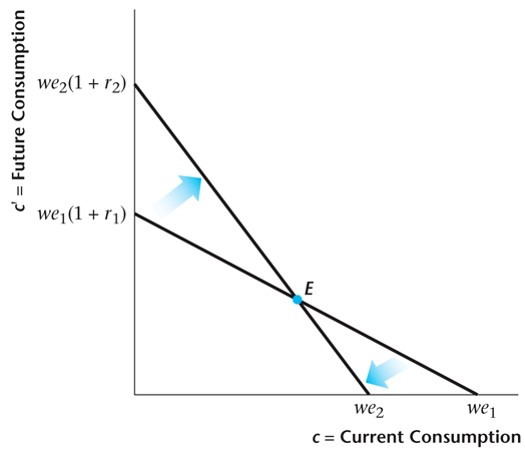
\includegraphics[width=\textwidth]{./figures/Figure9_12.jpg}
        \end{figure}
    \end{column}
    \begin{column}{0.5\textwidth}
        \begin{itemize}
            \item Recall $ \displaystyle  we = y - t + \frac{y' - t'}{1+r} $, $ r \uparrow  $ $ \Rightarrow  $ $ we \downarrow  $
            \item can do nothing: pivot around $ E $
            \item similar to \alert{wage increase} (slope $ \uparrow  $)
            \item income \& substitution effects (change in relative price)
            \item income effect depends on the sign of saving $ s $
        \end{itemize}
    \end{column}
\end{columns}
\end{frame}

\begin{frame}{Increase in Real Interest Rate: Effect on Lender ($s > 0$)}
\label{slide:Increase_in_Real_Interest_Rate__Effect_on_Lender}
    \begin{columns}
        \begin{column}{0.5\textwidth}
            \begin{figure}
                \caption{\scriptsize Figure 9.13  An Increase in the Real Interest Rate for a Lender}
                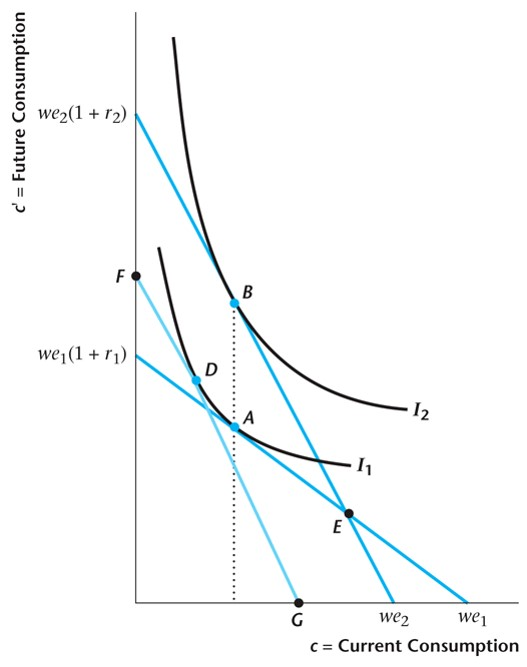
\includegraphics[width=\textwidth]{./figures/Figure9_13.jpg}
            \end{figure}
        \end{column}
        \begin{column}{0.5\textwidth}
            Let initial bundle be $ A $.
            \begin{itemize}
                \item \textbf{Substitution effect}: rotate from $ \overline{AE} $ to $ \overline{FG} $
                \begin{itemize}
                    \item $ \because r \uparrow  $, \alert{current consumption become more expensive} $ \Rightarrow  $ $ \red{c_{D} < c_{A}}, c'_{D} > c'_{A} $
                \end{itemize}
                \item \textbf{Income effect}: shift from $ \overline{FG} $ to $ \overline{BE} $
                \begin{itemize}
                    \item normality: $ \red{c_{B} > c_{D}}, c'_{B} > c'_{D} $
                    \item $ c' \uparrow $, $ \because $ both effects aligned
                    \item $ c $ and $ s = y - t - c $ are ambiguous, $ \because $ both effects contradict
                \end{itemize}
            \end{itemize}
        \end{column}
    \end{columns}
\end{frame}

\begin{frame}{Increase in Real Interest Rate: Effect on Borrower ($s < 0$)}
\label{slide:Increase_in_Real_Interest_Rate__Effect_on_Borrower}
    \begin{columns}
        \begin{column}{0.5\textwidth}
            \begin{figure}
                \caption{\scriptsize Figure 9.14  An Increase in the Real Interest Rate for a Borrower}
                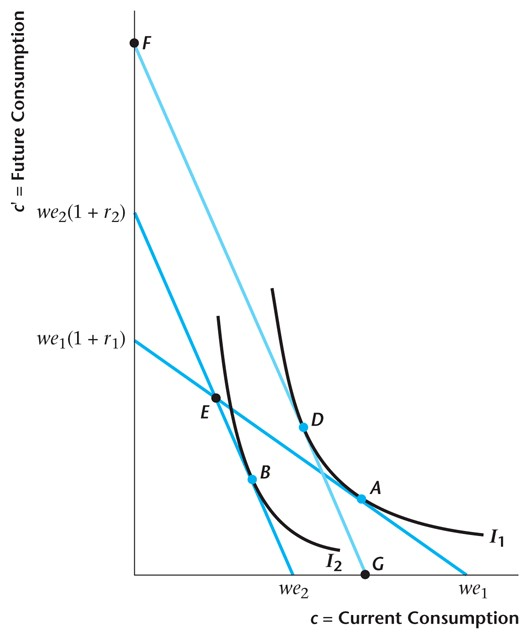
\includegraphics[width=\textwidth]{./figures/Figure9_14.jpg}
            \end{figure}
        \end{column}
        \begin{column}{0.5\textwidth}
            Let initial bundle be $ A $.
            \begin{itemize}
                \item \textbf{Substitution effect}: rotate from $ \overline{AE} $ to $ \overline{FG} $
                \begin{itemize}
                    \item $ \because r \uparrow  $, \alert{current consumption become more expensive} $ \Rightarrow  $ $ c_{D} < c_{A}, \red{c'_{D} > c'_{A}} $ [same as lender!]
                \end{itemize}
                \item \textbf{Income effect}: shift from $ \overline{FG} $ to $ \overline{BE} $
                \begin{itemize}
                    \item normality: $ c_{B} < c_{D}, \red{c'_{B} < c'_{D}} $ [opposite to lender!]
                    \item $ c, s \downarrow $, $ \because $ both effects aligned
                    \item $ c' $ is ambiguous, $ \because $ both effects contradict
                \end{itemize}
            \end{itemize}
        \end{column}
    \end{columns}
\end{frame}

\begin{frame}{Summary}
\label{slide:Summary}
    Both borrowers and lenders experience \alert{intertemporal substitution}:
    \begin{itemize}
        \item $ r \uparrow  $ $ \Rightarrow  $ cost of current consumption $ \uparrow  $ $ \Rightarrow  $ $ c \downarrow  $
        \item aggregate effect depends on the \alert{distribution} of borrowers and lenders
        \begin{itemize}
            \item $ \because $ both effects are in opposite directions
            \item important and active research topic in macro!
        \end{itemize}
        \item tendency for confounding income effects on borrowers and lenders to roughly cancel out, still \alert{effect on aggregate consumption} is not guaranteed.
    \end{itemize}
\end{frame}

\section{Competitive Equilibrium}
\label{sec:Competitive_Equilibrium}

\begin{frame}{Government in Two-Period Model}
\label{slide:Government_in_Two_Period_Model}
    Impose \alert{lump-sum tax} $ T $ and issue \alert{government bond} $ B $ to finance \alert{government spending} $ G $ in each period.
    \begin{itemize}
        \item government purchase $ G $ unit of good today and $ G' $ tomorrow,
        \item impose $ T $ and $ T' $ of lump-sum taxes to consumers, and
        \item Issue $ B $ unit of bond today and pay back $ ( 1+r ) B $ tomorrow.
    \end{itemize}
    Budget constraints:
    %
    \begin{align}
        \text{date 0}: \quad
            & G = T + B
        \\
        \text{date 1}: \quad
            & G' + ( 1+r ) B = T'
        \\
        \Rightarrow \text{lifetime budget constraint}: \quad
            & G + \frac{G'}{1+r} = T + \frac{T'}{1+r}
    \end{align}
    %
    Budget deficit is allowed in one period, but \textbf{must be repaid} in the future.
\end{frame}

\begin{frame}{Two-Period Competitive Equilibrium in Words}
\label{slide:Two_Period_Competitive_Equilibrium_in_Words}
A competitive equilibrium given \alert{government spending} and \alert{consumers' endowment} is a set of \textbf{endogenous quantities and prices} of \alert{current and future consumption}, \alert{current and future lump-sum taxes}, \alert{savings}, \alert{government bond}, as well as the \alert{real interest rate} such that
\begin{enumerate}
    \item Taken the real interest rate and lump-sum taxes as given, \textbf{consumers} maximized their lifetime utility subject to the intertemporal budget constraints.
    \item Taken the real interest rate as given, the intertemporal \textbf{government} budget constraint holds.
    \item The credit market clears determines the equilibrium real interest rate.
\end{enumerate}
\end{frame}

\begin{frame}{Two-Period Competitive Equilibrium in Math}
\label{slide:Two_Period_Competitive_Equilibrium_in_Math}
    A competitive equilibrium given exogenous quantities $\alert{ \{ G, G', Y, Y' \} }$, is a set of \textbf{endogenous quantities and prices} $ \green{\{ C, C', S, T, T', B, r \} }$
    \begin{enumerate}
        \item Taken \orange{$r$, $T$, and $ T' $}, \textbf{consumers} solve
        %
        \begin{equation*}
            \max_{\green{C, C'}} U( \green{C, C'} )
            \quad
            \text{subject to}
            \quad
            \green{C} + \frac{\green{C'}}{1+\orange{r}} = \alert{Y} - \orange{T} + \frac{\alert{Y'} - \orange{T'}}{1+\orange{r} }
        ,\end{equation*}
        %
        where solutions are $ C^{*}, C'^{*} $, and $ S^{*} = Y - T - C^{*} $.
        \item The \alert{present value} of \textbf{government budget constraint} holds:
        %
        \begin{equation*}
           \alert{G} + \frac{\alert{G'}}{1+\orange{r}}
           =
           \green{T} + \frac{\green{T'}}{1+\orange{r}}
        ,\end{equation*}
        %
        where government bond $ B $ is determined by $ B = G - T $.
        \item The \textbf{credit market clears}: $ S = B $ at the equilibrium interest rate $ r^{*} $.
    \end{enumerate}
\end{frame}

\begin{frame}{The Credit Market and GDP Accounting}
\label{slide:The_Credit_Market_and_GDP_Accounting}
    In \alert{one-period} model, firm and consumer interact in the \alert{labor market}.

    \orange{Here}, government and consumer interact in the \orange{credit market}.
    \begin{itemize}
        \item $ S $ is \alert{private saving}, and $ -B = S^{g} $ is \alert{public saving}
        \item closed economy: national net saving must equals $ 0 $, so $ S - B = 0 $.
        %
        \begin{align*}
            \text{current consumer budget:} \quad
                & S = Y - T - C
            \\
            \text{with current gov budget:} \quad
                & S = Y - ( G-B ) - C
            \\
            S = B: \quad
                & Y = C + G
            \\
            \text{future consumer budget:} \quad
                & ( 1+r ) S = C' + T' - Y'
            \\
            \text{with future gov budget:} \quad
                & ( 1+r ) S = C' + ( G' + ( 1+r ) B ) - Y'
            \\
            S = B: \quad
                & Y' = C' + G'
        \end{align*}
        %
    \end{itemize}
\end{frame}

\begin{frame}{An Example}
\label{slide:An_Example}
    Suppose $ G = G' = T = T' = B = 0 $, i.e., government is ignored, then
    \begin{itemize}
        \item \textbf{consumer}: let $ U( C, C' ) = \ln C + \ln C' $, and $ Y = Y' = 1 $,
        %
        \begin{equation*}
            \max_{C, C'} \ln C + \ln C' \quad \text{subject to} \quad C + \frac{C'}{1+r} = 1 + \frac{1}{1+r}
        \end{equation*}
        %
        \item FOC:
        %
        %
        \begin{align*}
            MRS_{C, C'} = \frac{C'}{C} = 1+r \quad \Rightarrow \quad
                & C + \frac{(1+r)C}{1+r} = \frac{2+r}{1+r}
            \\
            \quad \Rightarrow \quad
                & 2C = \frac{2+r}{1+r} \Rightarrow C^{*} = \frac{2+r}{2( 1+r )}
        \end{align*}
        %
        \item \textbf{credit market clear:}
        %
        \begin{equation*}
            S = B = Y - T - C^{*} = 1 - 0 - \frac{2+r}{2( 1+r )} = 0 \Rightarrow r^{*} = 0 \Rightarrow C = C' = 1
        \end{equation*}
        %
    \end{itemize}
\end{frame}

\section{Ricardian Equivalence}
\label{sec:Ricardian_Equivalence}

\begin{frame}{Ricardian Equivalence}
\label{slide:Ricardian_Equivalence}
    In this model, the timing of taxes is \textbf{neutral}: no effect on the real interest rate or on the consumption of individual consumers.

    Recall consumer and government budget constraint:
    %
    \begin{align*}
        \text{government}: \quad
            & G + \frac{G'}{1+r} = T + \frac{T'}{1+r}
        \\
        \text{consumer}: \quad
            & C + \frac{C'}{1+r} = Y + \frac{Y'}{1+r} - \left( T + \frac{T'}{1+r} \right)
        \\
            &  \qquad \qquad \qquad = Y + \frac{Y'}{1+r} - \left( G + \frac{G'}{1+r} \right)
    \end{align*}
    %
    Therefore, for any tax scheme such that government budget constraint holds, there's no effect on $ r $, $ C $ and $ C' $.
\end{frame}

\begin{frame}{Ricardian Equivalence in Graph}
\label{slide:Ricardian_Equivalence_in_Graph}
    \begin{columns}
        \begin{column}{0.5\textwidth}
            \begin{figure}
                \caption{\scriptsize Figure 9.16  Ricardian Equivalence with a Cut in Current Taxes for a Borrower}
                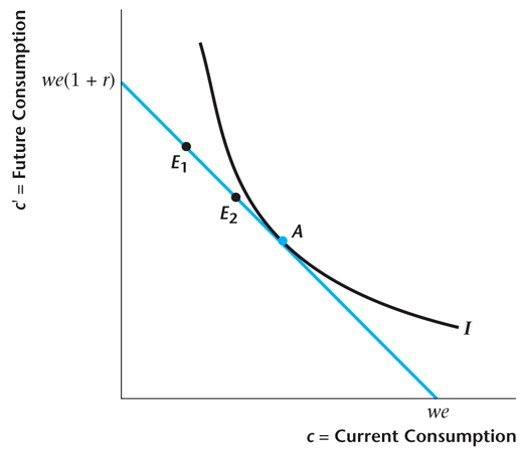
\includegraphics[width=\textwidth]{./figures/Figure9_16.jpg}
            \end{figure}


        \end{column}
        \begin{column}{0.5\textwidth}
            Suppose under tax scheme $ ( T, T' ) $, consumer:
            \begin{itemize}
                \item has endowment point $ E_{1} $
                \item chooses optimal bundle $ A $
            \end{itemize}
            If there's a tax cut scheme $ ( \tilde{T}, \tilde{T'} ) $ such that $ ( G, G' ) $ remain the same,
            \begin{itemize}
                \item lower current taxes $ ( \tilde{T} < T ) $
                \item but higher future taxes $ ( \tilde{T'} > T' ) $
            \end{itemize}
            Then consumer has endowment $ E_{2} $, but still choose optimal bundle $ A $.
        \end{column}
    \end{columns}
\end{frame}

\begin{frame}{Ricardian Equivalence and Credit Market}
\label{slide:Ricardian_Equivalence_and_Credit_Market}
    \begin{columns}
        \begin{column}{0.5\textwidth}
            \begin{figure}
                \caption{\scriptsize Figure 9.17  Ricardian Equivalence and Credit Market Equilibrium}
                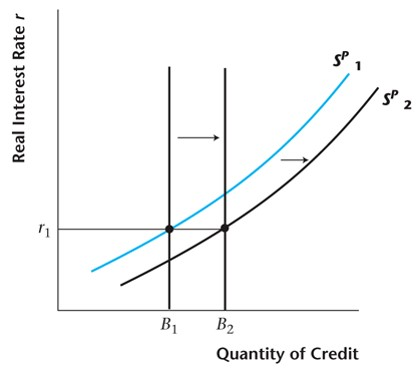
\includegraphics[width=\textwidth]{./figures/Figure9_17.jpg}
            \end{figure}
        \end{column}
        \begin{column}{0.5\textwidth}
            Following the tax cut in last slide,
            \begin{itemize}
                \item $ T \downarrow  $ $ \Rightarrow  $ larger deficit today
                \item Recall $ B = G - T $, $ B \uparrow  $, more bonds today (demand $ \uparrow  $)
                \item Recall $ S = Y - T - C $, $ S \uparrow  $, more private saving today (supply $ \uparrow  $)
                \item Ricardian Equivalence: both shifts \alert{exactly} offsets, $ r_{2} = r_{1} $
                \item Recall PIH: tax cut is $ 100\% $ temporary!
            \end{itemize}
        \end{column}
    \end{columns}
\end{frame}

\begin{frame}{When Will Ricardian Equivalence fail?}
\label{slide:When_Will_Ricardian_Equivalence_fail_}
    This is an extreme result! It provides a useful \alert{benchmark} to consider richer settings. What can change to ``undo'' this result?
    \begin{enumerate}
        \item \textbf{distribution of tax burden:} consider a case of this model with $ N $ consumers, labeled $ i = 1, \ldots N$. Assume that $ T = \sum_{i=1}^{N} t_{i} $, and consumer $ i $ pays $ t_{i} $.
        \begin{itemize}
            \item Everyone pays different $ t_{i} $! What if tax cut not apply to everyone?
        \end{itemize}
        \item \textbf{consumer lives the whole time:} government can ``kick the can'' until long in the future, when current generation is retired or dead.
        \begin{itemize}
            \item redistribution of wealth across generations, social security
        \end{itemize}
        \item \textbf{distorting taxes:} lump sum not feasible, but proportional distort
        \item \textbf{imperfect credit market:} borrowing and lending is often ``\alert{frictional}''
        \begin{itemize}
            \item example: different rates on borrowing and saving, many others!
        \end{itemize}
    \end{enumerate}
\end{frame}

\end{document}

